\documentclass[xetex,mathserif,serif]{beamer}
\usepackage{polyglossia}
\setdefaultlanguage[babelshorthands=true]{russian}
\usepackage{minted}
\usepackage{tabu}

\useoutertheme{infolines}

\usepackage{fontspec}
\setmainfont{FreeSans}
\newfontfamily{\russianfonttt}{FreeSans}

\setbeamertemplate{blocks}[rounded][shadow=false]

\definecolor{links}{HTML}{2A1B81}
\hypersetup{colorlinks,linkcolor=,urlcolor=links}

\tabulinesep=0.7mm

\newcommand{\attribution}[1] {
	\vspace{-5mm}\begin{flushright}\begin{scriptsize}\textcolor{gray}{\textcopyright\, #1}\end{scriptsize}\end{flushright}
}

\title{Диаграммы классов UML}
\author[Юрий Литвинов]{Юрий Литвинов \newline \textcolor{gray}{\small\texttt{yurii.litvinov@gmail.com}}}

\date{12.02.2020г}

\begin{document}
	
	\frame{\titlepage}

	\section{Обратная связь по домашке}

	\begin{frame}
		\frametitle{Обратная связь по домашке}
		\begin{itemize}
			\item Запуск из консоли
			\begin{itemize}
				\item Инструкция по сборке/запуску в README
			\end{itemize}
			\item CI под Windows и Linux
			\item Внимательно читайте условие!
			\begin{itemize}
				\item Нет способа определить, вы не заметили какой-то пункт или злонамеренно решили его не делать
			\end{itemize}
			\item Реализация exit
			\item Поток ошибок
		\end{itemize}
	\end{frame}

	\section{BPMN}

	\begin{frame}
		\frametitle{Нанорассказ про BPMN}
		\begin{center}
			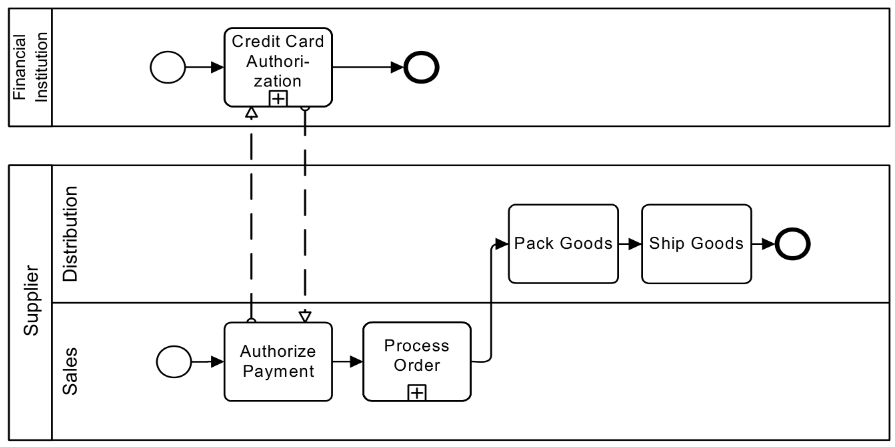
\includegraphics[width=0.9\textwidth]{bpmnExample.png}
			\attribution{OMG BPMN 2.0 Specification}
		\end{center}
	\end{frame}

	\section{CASE-системы}

	\begin{frame}
		\frametitle{Computer-Aided Software Engineering}
		\begin{itemize}
			\item В 80-е годы термином CASE называли всё, что помогает разрабатывать ПО с помощью компьютера
			\begin{itemize}
				\item Даже текстовые редакторы
			\end{itemize}
			\item Теперь --- прежде всего средства для визуального моделирования (UML-диаграммы, ER-диаграммы и т.д.)
			\item Отличаются от графических редакторов тем, что ``понимают'', что в них рисуют
			\item Нынче чаще используются термины ``MDE tool'', ``UML tool'' и т.д.
		\end{itemize}
	\end{frame}

	\begin{frame}
		\frametitle{Типичная функциональность CASE-инструментов}
		\begin{itemize}
			\item Набор визуальных редакторов
			\item Репозиторий
			\item Набор генераторов
			\item Текстовый редактор
			\item Редактор форм
			\item Средства обратного проектирования (reverse engineering)
			\item Средства верификации и анализа моделей
			\item Средства эмуляции и отладки
			\item Средства обеспечения командной разработки
			\item API для интеграции с другими инструментами
			\item Библиотеки шаблонов и примеров
		\end{itemize}
	\end{frame}

	\begin{frame}
		\frametitle{Примеры CASE-инструментов}
		\begin{itemize}
			\item ``Рисовалки''
			\begin{itemize}
				\item Visio
				\item Dia
				\item SmartDraw
				\item Creately
			\end{itemize}
			\item Полноценные CASE-системы
			\begin{itemize}
				\item Enterprise Architect
				\item Rational Software Architect
				\item MagicDraw
				\item Visual Paradigm
				\item GenMyModel
			\end{itemize}
			\item Забавные штуки
			\begin{itemize}
				\item \url{https://www.websequencediagrams.com/}
				\item \url{http://yuml.me/}
				\item \url{http://plantuml.com/}
			\end{itemize}
		\end{itemize}
	\end{frame}

	\section{Диаграммы классов и объектов UML}

	\begin{frame}
		\frametitle{Диаграммы классов UML}
		\begin{center}
			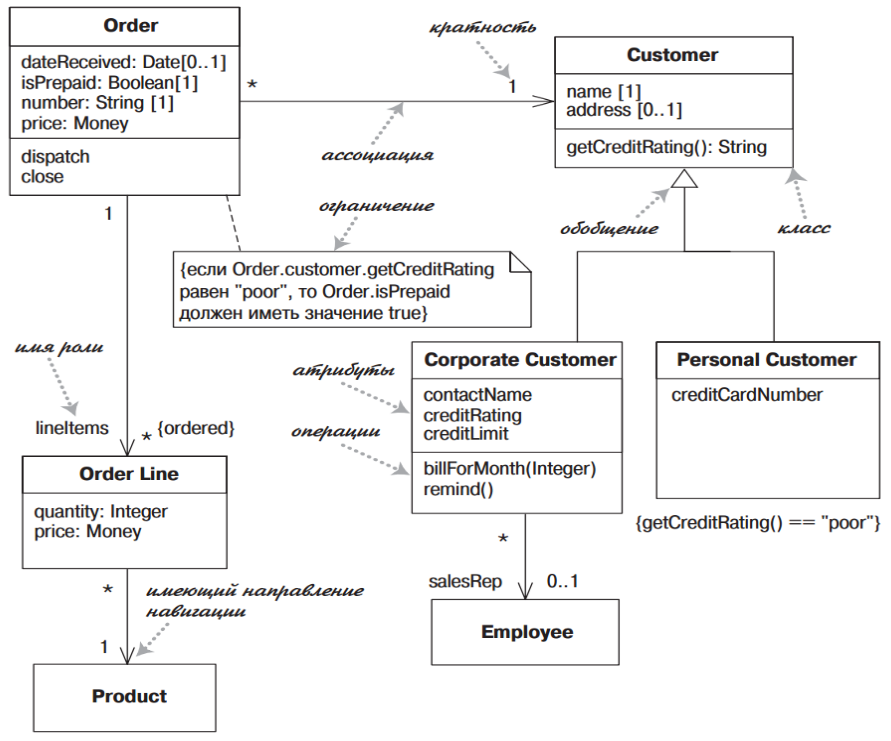
\includegraphics[width=0.7\textwidth]{umlClassDiagram.png}
		\end{center}
	\end{frame}

	\begin{frame}
		\frametitle{Свойства}
		\begin{columns}
			\begin{column}{0.3\textwidth}
				\begin{center}
					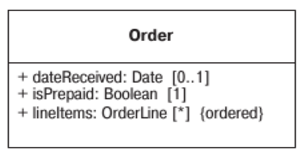
\includegraphics[width=0.8\textwidth]{attributes.png}

					Атрибуты
				\end{center}
			\end{column}
			\begin{column}{0.7\textwidth}
				\begin{center}
					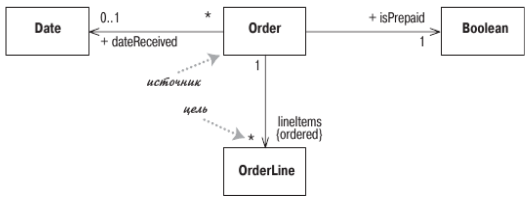
\includegraphics[width=0.7\textwidth]{associations.png}

					Ассоциации
				\end{center}
			\end{column}
		\end{columns}
		\bigskip
		Синтаксис:
		\begin{itemize}
			\item видимость имя: тип кратность = значение по умолчанию \{строка свойств\}
			\item Видимость: + (public), - (private), \# (protected), \char`~ (package)
			\item Кратность: 1 (ровно 1 объект), 0..1 (ни одного или один),\newline * (сколько угодно), 1..*, 2..*
		\end{itemize}
	\end{frame}

	\begin{frame}
		\frametitle{Агрегация и композиция}
		Агрегация – объект ``знает'' о другом (не управляет его временем жизни, имеет на него ссылку или указатель)
		\begin{center}
			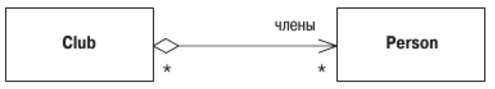
\includegraphics[width=0.5\textwidth]{aggregations.png}
		\end{center}
		Композиция --- объект владеет другим объектом (управляет его временем жизни, хранит его по значению или по указателю, делая delete)
		\begin{center}
			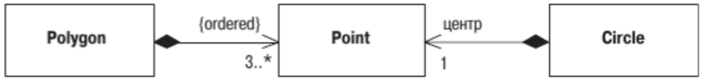
\includegraphics[width=0.7\textwidth]{compositions.png}
		\end{center}
		Уточнение обычной ассоциации, используется только если очень надо
	\end{frame}

	\begin{frame}
		\frametitle{Прочее}
		\begin{columns}
			\begin{column}{0.5\textwidth}
				\begin{center}
					Интерфейсы

					\bigskip
					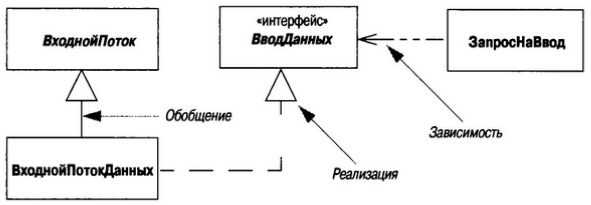
\includegraphics[width=0.9\textwidth]{interfaces1.png}

					\bigskip
					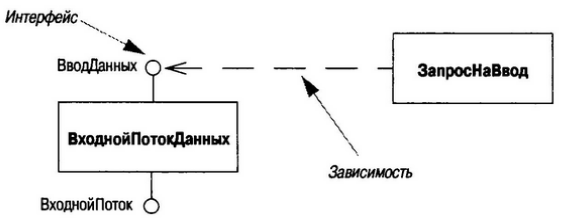
\includegraphics[width=0.9\textwidth]{interfaces2.png}
				\end{center}
			\end{column}
			\begin{column}{0.5\textwidth}
				\begin{center}
					Зависимости

					\bigskip
					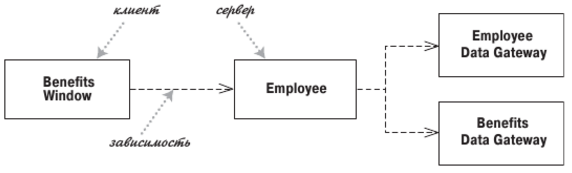
\includegraphics[width=0.9\textwidth]{dependencies.png}
					\bigskip

					Шаблоны

					\bigskip
					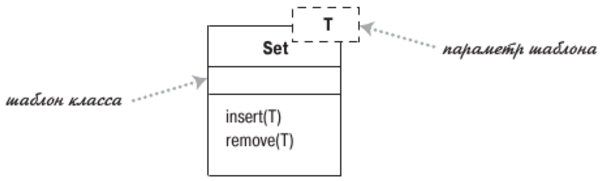
\includegraphics[width=0.9\textwidth]{templates.png}
				\end{center}
			\end{column}
		\end{columns}
	\end{frame}

	\begin{frame}
		\frametitle{Диаграммы объектов}
				\begin{columns}
			\begin{column}{0.5\textwidth}
				\begin{itemize}
					\item snapshot структуры классов во время выполнения
					\item Используются обычно чтобы пояснить диаграмму классов
					\item Полезны на этапе анализа предметной области, ещё до диаграмм классов
				\end{itemize}
			\end{column}
			\begin{column}{0.5\textwidth}
				\begin{center}
					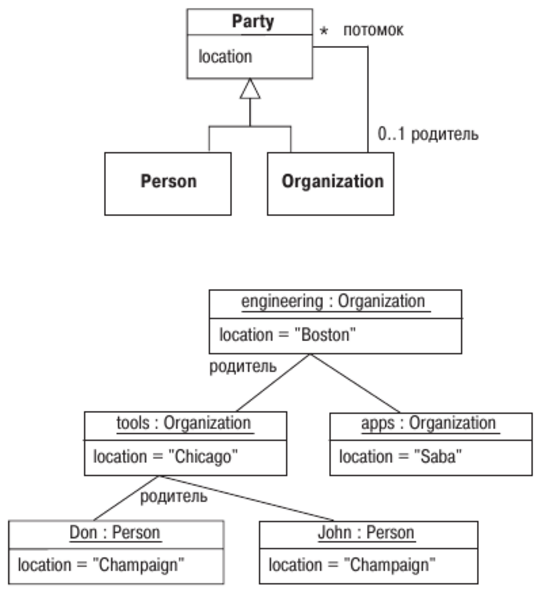
\includegraphics[width=\textwidth]{objectsDiagram.png}
				\end{center}
			\end{column}
		\end{columns}
	\end{frame}

	\section{Задания}

	\begin{frame}
		\frametitle{Домашнее задание: cd, ls}
		\begin{itemize}
			\item Реализовать команды \textbf{ls} и \textbf{cd} на базе кода одногруппника
			\begin{itemize}
				\item Обе команды могут принимать 0 или 1 аргумент
				\item Не забывайте про юнит-тесты
			\end{itemize}
			\item Написать ревью на архитектуру оного одногруппника, указав, что оказалось удобным, а что неудобным при реализации, что можно было бы улучшить
			\item Сделать fork на GitHub, выложить изменения туда и сделать пуллреквест в свой форк
			\begin{itemize}
				\item Если ``жертва'' не против, можно и в исходный репозиторий
			\end{itemize}
			\item Реализация, в которой надо сделать команды, определяется циклическим сдвигом на \textbf{3} вниз по списку на HwProj
		\end{itemize}
	\end{frame}

	\begin{frame}
		\frametitle{Задание на остаток пары}
		\begin{itemize}
			\item Нарисовать диаграмму классов UML для своего решения CLI, как оно есть
			\item Обращать внимание на синтаксис UML и читаемость диаграммы
			\item Как будет готово, позвать меня и показать
			\item Не пытаться рисовать методы, кроме самых важных
			\item Не рисовать все поля --- надо успеть до конца пары
		\end{itemize}
	\end{frame}

\end{document}
